\documentclass[12pt]{article}

%margin
\usepackage[left=1cm, right=1cm, top=2.5cm, bottom=2.5cm]{geometry}

%symbols, fonts
\usepackage{amsmath, amssymb, amsfonts}

%cross ref
\usepackage{cite, hyperref} 

%affiliation
\usepackage{authblk}

%graphic
\usepackage{graphicx}


\newtheorem{thm}{Theorem}
\newtheorem{asm}{Assumption}

\author[1]{Jaemin Oh}
\affil[1]{Department of Mathematical Sciences, KAIST}

%1.5 line space
\linespread{1.5} 

\title{Causal temperature-mortality relationship using time-series data}

\begin{document}

\maketitle
%\tableofcontents

\abstract{In this paper, 
we analyzed the causal relationship between the ambient temperature and all-cause mortality 
in South Korea using the regional time-series data.}

\section{Introduction}

Identifying the causal effect of the ambient temperature on human health is 
an important research topic due to global warming and climate change.
The best way to identify the causal effect would be observing
how the change of the ambient temperature affects 
the change of total death count in one region under Ceteris Paribus condition.
Note that, perfect Ceteris Paribus condition is only possible
when we can access to the parallel world that 
another treatment would have been assigned while other variables are the same.
However, it is definitely impossible.
Therefore, we must identify the causal effect by analyzing time series data
which is a record of date, daily mean temperature, and daily total death count in a region.
Analysis of this time series data is a challenging task, because of several reasons:
the ambient temperature is continuous treatment, so the size of the effect may be differ for each temperature;
the effect of the ambient temperature may be delayed;
serial correlation of daily mean temperature makes difficult to separate instant and delayed effect;
daily death count has a temporal trend, it increases as the population size increases.
In previous studies (Gapsparrini, Guo, etc), these difficulties were addressed by 
the combination of the DLNM framework\cite{dlnm2010}
and the quasi-Poisson regression\cite{quasipoisson} that produces exposure-response surface
$\mu : (w, l) \mapsto \mu(w,l)$ where $w$ is the ambient temperature and $l$ is a time lag.

The DLNM framework has many advantages:
it summarizes the information of the RR curve by spline coefficients,
so multivariate meta-analysis is possible;
lagged effect can be easily identified;
well developed R-package is available\cite{dlnm2010R}.
These advantages make the DLNM framework popular in environmental epidemiology,
especially for the topic of temperature-mortality relationship.
However, model selection in the DLNM framework is quite complicated 
so we may say that it is susceptible to model misspecification\cite{gasparrini2016}.
It eliminates temporal trend of death count by fitting additional spline for each year,
and it requires determination of degrees of freedom for each spline base.
Also we never know the exact degrees of freedom 
and placement of knots for spline bases of the ambient temperature.
Those values can be determined based on the previous studies, 
or Akaike information criterion\cite{dlnm2010}.

There was a debate on air pollution study 
that usual regression approach to analyze the health effect of particulate matter 
does not inform causality very well\cite{dominici2019sci}.
One reason is, as stated above, model selection problem
and another reason is mixing of design stage and analysis stage.
Rubin said that final outcome data should not be used in design stage without some exceptions\cite{rubin2008}.
Here, in the context of the DLNM framework,
design stage is fitting splines for each year to adjust confounding bias, 
and analysis stage is fitting the cross basis to the data.
The DLNM framework is done by doing Poisson regression to the data,
stated concerns about regression analysis is still valid in temperature-mortality relationship.

A model that separates design and analysis stage is Rubin causal model (RCM)\cite{holland1986}.
It is about how to compare counterfactual outcomes of another parallel world, 
without access to the parallel world under suitable assumptions.
The potential outcome framework was first introduced 
to analyze the data of randomized experiments\cite{rubin1974},
but now widely used in observational studies\cite{wu2020sciadv}.
Furthermore, the potential outcome framework is more free 
to the problem of model misspecification than the traditional approach, 
because it is in some sense "semi-parametric" 
that does not require parametric model for outcome generating process.\cite{angrist2018} 
So in this paper, we used potential outcome framework 
to estimate logRR curve of the ambient temperature.

Usually, the potential outcome framework is applied to individual level data. 
For example, analyzing treatment effect of new medicine. 
However, it is hard to earn individual level data for temperature-mortality relationship,
to say that the true cause of death was the ambient temperature, 
and to analyze short-term effect on individual level. 
Therefore we used regional data instead of individual level data.

\section{Method}

The state of a region at time $t$ can be described by $(Y_t, W_t, C_t)$ 
where $Y_t$ is a vector of outcome, $W_t$ is a treatment, and $C_t$ is a vector of confounders.

In regression settings, we usually have fitted the model:
\[
	g\left( \mathbb{E}\left[ Y_t \lvert W_t, C_t \right] \right) = s(W_t)\beta + \eta(C_t)\gamma
\]
where $g$ is a link function and $(s,\gamma)$ are bases of function space, such as spline bases.
However, as described before, regression approaches inform weak causality 
because of mixing of design and analysis stages and model selection problem.
To deal with this problem, we used potential outcome framework with nonparametric effect estimator.

\subsection{Conceptual framework}

What would be the value of $Y_t$ if $W_t = w'$ had been observed instead of $W_t = w$?
The outcome of this counterfactual imagination is called potential outcome and written as $Y_t(w')$.
If we know true value of $Y_t(w)$ and $Y_t(w')$, we can get the relative risk of $w$ against $w'$ by
\[
	\frac{Y_t(w)}{Y_t(w')} \text{ or } 
	\frac{\mathbb{E}\left[ Y_t(w) \right]}{\mathbb{E}\left[ Y_t(w') \right]}.
\]
However, we never know the true $Y_t(w)$, due to its counterfactual nature.
This is called the fundamental problem of causal inference\cite{holland1986}.

There has been many studies to address this problem.
In (marginally) randomized experiment, 
$\mathbb{E}[Y(w)]$ can be estimated from observed data\cite{rubin1974}.
In observational studies, 
one can estimate causal estimand $\mu(w) = \mathbb{E}[Y(w)]$ by preprocessing the data to approximate randomization 
e.g., inverse probability weighting, standardization, matching\cite{rosenbaum1983}.
Among those techniques, 
common assumptions that makes it possible to estimate the causal estimand are below:

\begin{asm}[Consistency]\hfill

	Potential outcome for observed treatment is equal to the observed outcome.
	That is, $Y_t(W_t) = Y_t$.
\end{asm}

\begin{asm}[Positivity]\hfill
	Discrete treatment:
	For all $w$ and $C_t$, $p(w\lvert C_t) = Pr\left ( W_t = w \lvert C_t\right ) \in (0, 1)$.

	Continuous treatment:
	For all $w$ and $C_t$, $p(w\lvert C_t) > 0$ where $p(w\lvert C_t)$ is a conditional density.
\end{asm}


\begin{asm}[Weak Unconfoundedness] \hfill

	For all $w$, $Y_{t}(w) \perp W_t \lvert C_t$.
\end{asm}


Positivity assumption says all treatments are possible for each confounder.
Weak unconfoundedness assumption says
conditional on current confounders, potential outcomes are already determined.
With these, the causal estimand can be calculated as
\[
	\begin{split}
		\mathbb{E}\left[ Y_t\frac{1_{(W_t = w)}}{p(w\lvert C_t)} \right]
		& = \mathbb{E}\left[ \mathbb{E}\left( Y_t(w) \frac{1_{(W_t = w)}}{p(w\lvert C_t)} \lvert C_t\right)\right]\\
		& = \mathbb{E}\left[ Y_t(w)\frac{\mathbb{E}\left( 1_{(W_t = w)}\lvert C_t \right)}{p(w\lvert C_t)} \right]\\
		& = E\left[ Y_t(w) \right].
	\end{split}
\]
This is called "inverse probability weighting" (IPW).
Thus, a natural estimator of the causal estimand is
\[
	\hat{\mu}(w) = \frac{1}{T}\sum_{t = 1}^T Y_t \frac{1_{(W_t = w)}}{p(w\lvert C_t)}.	
\]
Note that the first equality comes from the interated expectation formula and consistency assumption,
the second equality comes from weak unconfoundedness assumption,
and the last equality is due to the definition of $p(w\lvert C_t)$.
By positivity assumption, we can divide by $p(w\lvert C_t)$.

Still, we need to estimate $p(w\lvert C_t)$ since it is unknown to us in general.
When the treatment is binary, $p(w\lvert C_t)$ is called propensity score,
and it is used to adjust for confounding bias\cite{rosenbaum1983}.
Propensity score can be extended to 
"generalized propensity score" (GPS) for categorical or continuous treatment\cite{imbens2000}.
For binary treatment, one can estimate propensity score by fitting logit model to data.
For categorical or continuous treatment, GPS can be estimated by fitting ordered probit model or boosting.

PS and GPS have two nice properties\cite{rosenbaum1983, hirano2004}.
The first one is balancing property, which means that conditional on the same PS (or GPS),
treatment and covariates are independent.
The second one is PS-unconfoundedness, 
which means that conditional independence of potential outcome and treatment given PS.
PS-unconfoundedness is implied by balancing property and unconfoundedness.
These properties are the basis of propensity score based matching methods.
But in this paper, we used inverse probability weighting so these properties are not needed.

The main reason why we use inverse probability weighting by GPS is to achieve covariate balance.
In randomized experiment, distribution of covariates are similar across each treated group.
However, we are now dealing with observational data 
so we are looking forward to achieve covariate balance on pseudo-population generated by
imposing appropriate weights to each observation.
One criteria for covariate balance is the absolute correlation (AC)\cite{gpsboosting2015}.
If treatment and covariates are independent, then their correlation must be zero.
So, small value of AC can be an one possible evidence of covariate balance.
Usually, AC with $ <0.1 $ is considered as acceptible.

In fact, matching method to adjust confounding bias is available for continuous treatment data\cite{wu2020arxiv}.
However, in our case, extreme temperatures are rarely observed,
so matching estimator can heavily depend on such observations and can lead exaggerated effect estimate.
Instead, in IPW method, too large weight is trimmed so it will produce less exaggerated estimate
compared to the matching method.

\section{Application}

(DATA DESCRIPTION)

For $i = 1, \dots, N$ and $t = 1, \dots, T$, 
let $(Y_{i,t}, W_{i,t}, C_{i,t})$ be information of $i$-th region at time $t$.
$Y$ is daily total death count, $W$ is daily mean temperature 
and $C$ is (year, month, the week of year, the day of year).
We rounded daily mean temperature to integer value.
In the next subsection in which we concentrate on single time series, 
we will drop $i$ to simpify the notation.

\subsection{Single series estimate}

The first stage is design stage to adjust for time confounding.
We adjusted confounding bias by stabilized inverse probability weighting\cite{sipw2010}
that assign weights
\[
	q_t = \min{ \left \{ \frac{p(W_t \lvert C_t)}{p(W_t)}, 10 \right \} }
\]
to each obsevation.
Here, we don't know true probability densities,
so we instead used estimated values.
One can use normal density as denominator $p(W_t)$,
but we used relative frequency as the denominator
since weighting method with relative frequency achieved 
lower absolute correlation in this application. (report the difference)
We trimmed weights bigger than $10$ by $10$,
because some estimated weights were too large so
effect estimate was heavily dependent to those observations.

To estimate the numerator $p(W_t \lvert C_t)$, 
we assumed that the conditional distribution of treatment given covariates is a normal distribution, i.e.
\[ 
	W\lvert C \sim N(m(C), \sigma(C)^2) 
\] 
where $m(C)$, and $\sigma(C)$ are some functions of $C$.
Since they are unknown in general, we should estimate them. 
The mean $\hat{m}(C)$ is estimated by boosting, 
and the standard deviation $\hat{\sigma}(C)$ is estimated by boosting residuals\cite{hirano2004, gpsboosting2015}.
Hyperparameters such as depth of tree, shrinkage, and the number of trees are determined
to minimize the absolute correlation. (report them)

We calculated absolute correlation (AC)\cite{gpsboosting2015} 
to see whether the covariate balance is achieved.
Let $c_t$ be a component of $C_t$, then absolute correlation with weight $q_t$ is
the absolute value of Pearson correlation coefficient between $c_t$ and $W_t$,
regarding each observation as $q_t$ observations with the same values.

After covariate balance is acheived (for example, AC$<0.1$), 
we estimated the causal effect by Horvitz-Thompson estimator with stabilized weights,
\[
	\hat{\mu}(w) = \frac{\sum_{t = 1}^T q_t Y_t 1_{(W_t = w)}}{\sum_{t = 1}^T q_t 1_{(W_t = w)}}
\]
With $\hat{\mu}(w)$, we calculaated logRR curve by $\log\hat{\mu}(w) - \log \hat{\mu}(20)$.
Uncertainty of logRR curve is quantified by Moving Block Bootstrapping (MBB)\cite{mbb1989}.
In the bootstrap procedure, we did not fit gps model repeatedely for each bootstrap sample
since we need to re-sample the pseudo-population itself that acheives covariate balance.

In fact, asymptotic confidence interval can be calculated 
if we concentrate on risk difference instead of risk ratio.
However, there is no known result about asymptotic distribution of risk ratio.
The reason why we care about the relative risk is
1) consistency to the previous studies
2) that the population sizes differ across regions.
If we consider the risk difference, then additional suitable normalizing step will be required.

\subsection{Pooling estimates}

(Assumption 4) - independence of regions

For each region $i$, we estimated $\hat{\mu}_i(w)$ in the previous section.
To obtain aggregated estimate,
we assumed
\[
	\hat{\mu}_i(w) = \mu(w) + \epsilon_i + \tau,
\]
where $\epsilon_i \sim N(0, S_i)$ is within study error and $\tau \sim N(0, V)$ is between study error.
$S_i$ is estimated by bootstrap,
so estimation of $V(\tau)$ remains.
We used R package 'mixmeta' to obtain pooled estimate,
which is the weighted average of region specific effect estimate
where weight is inversely proportional to the variance $S_i + V$ of estimator.
Precision of pooled estimator is sum of precisions of region specific estimator.
Confidence interval is obtained by adding (or subtracting) 
$1.96$ times of pooled standard deviation $\hat{\sigma}$ to pooled logRR curve.

\subsection{Result}

To compare estimate obtained above to the previous studies, we fitted DLNM to our data.
For temperature dimension, 
we used quadratic B-spline, and placed knots at 10th, 75th, 90th quantiles.
For lag dimension,
we considered $21$ lags, used natural B-spline, and placed $3$ knots at equally spaced log values.
For temporal trend adjustment,
we fitted additional natural B-spline with $8$ degrees of freedom for each year.

In figure 1,
the upper left panel is a logRR curve obtained under the DLNM framework;
the upper right panel is obtained by applying potential outcome framework;
the lower left panel is smoothed version of upper right pannel (kernel: Gaussian, bandwidth: $6$);
the lower right pannel is a logRR curve without adjusting temporal trend under the DLNM framework.

The estimated logRR curve of the lower right panel has exaggerated values at extreme temperatures,
compared to the upper left panel.
Since the model of the lower right panel does not consider temporal trend,
the difference between two panels comes from autocorrelation of outcome variable.

The logRR curve of the upper right panel is spiky,
because we estimated it by model free method, so it heavily depends on the observations.
For the most cold temperature, 
we can see that the confidence interval is narrow compared to the most hot temperature.
This is because there is only one such observation,
so uncertainty captured by bootstrap is due to the variation of effect estimate at the reference temperature.

In the lower left pannel, we applied kernel smoothing to our estimate to remove spikes.
The smoothed curve and the curve of the upper left panel have similar values 
compared to the curve of the lower right panel.
From this point of view, 
we may say potential outcome framework can adjust temporal confounding bias in some extent.
Moreover, we don't know what is the true logRR curve,
but we may insist that the logRR curve obtained from potential outcome framework is more general
in the sense that it becomes similar to the curve of DLNM after kernel smoothing.

\begin{figure}
	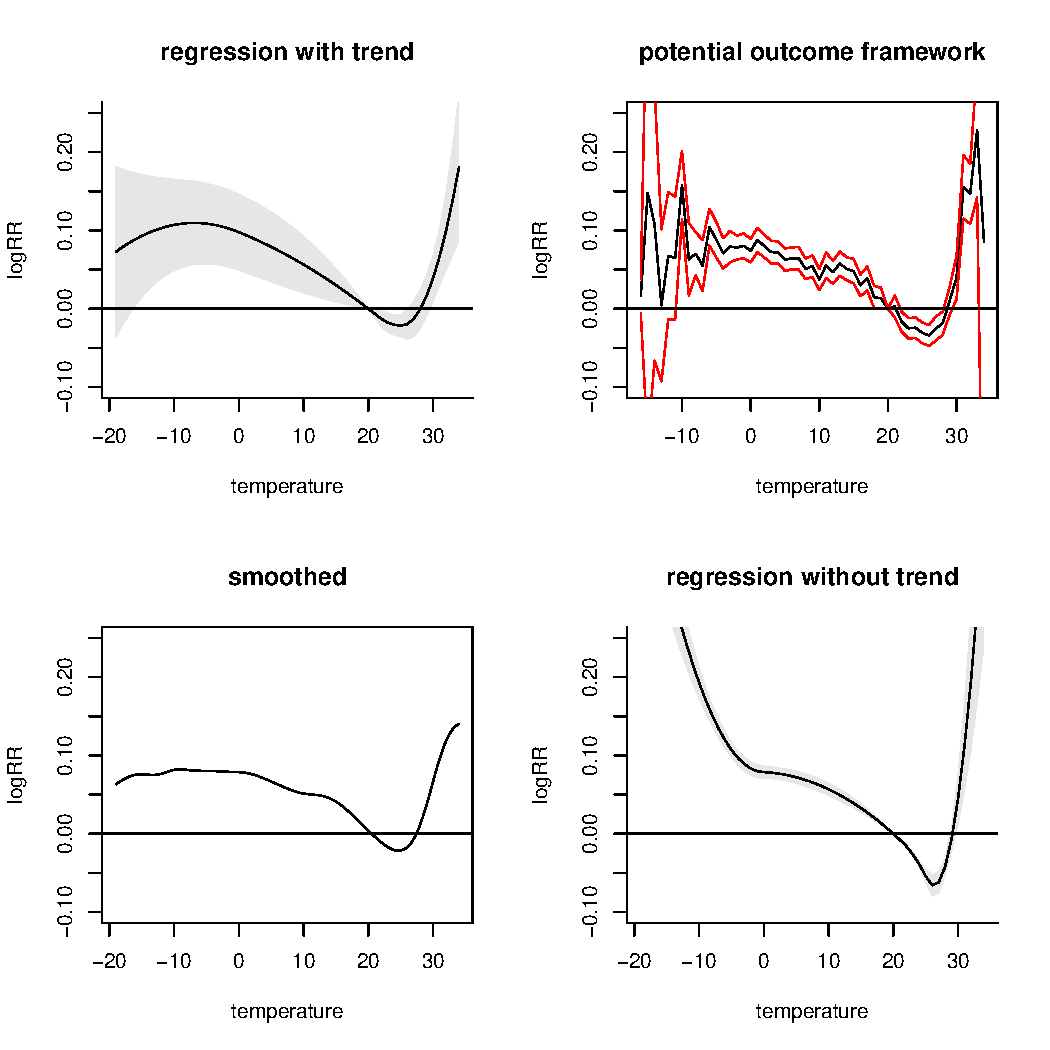
\includegraphics[width = \textwidth]{figures/main1.pdf}
	\caption[Figure 1.]{Estimated overall effect. 
	For extreme hot or cold temperature, estimated effects have quite large uncertainties.}
\end{figure}

\section{Discussion}

In the extent of my knowledge, there has been no studies to analyze the short term relationship 
between the ambient temperature and the all-cause mortality using the potential outcome framework.
In this work, the causal link between the ambient temperature and mortality 
is found under the potential outcome framework.
Consistency between new approach and existing regression method reinforces
usefulness of regression method, and adds an evidence of causal relationship found by previous studies.
However, there are some limitations to overcome.


\subsection{Limitation}

In this framework, we could not do several analyses that the DLNM framework can do:
lagged effect analysis, meta-regression and theoretical confidence interval.

The DLNM framework produces exposure-response surface with treatment dimension and lag dimension.
Therefore, we can easily measure the lagged effect of any treatment level after obtaining the surface.
In contrast, we estimated the effect of the treatment by using the current outcome variable.
This can produce only exposure-response curve, 
since we don't use any information about lagged treatment or lagged outcome.
Thus our approach does not have ability to measure the lagged effect of the treatment.
There is a method to measure the lagged effect of the treatment in a single time series\cite{bojinov2019}.
However, this paper is for binary (sequential) treatment 
so it is hard to be directly applied to continuous treatment case,
because of the curse of dimensionality.
With maximum lag $L$, the number of combinations of possible treatment path is $2^{L+1}$ for binary case
but there are more than $50$ categories of daily mean temperature 
so the number of treatment path exceeds $50^{L+1}$.
Even if $L = 2$, 
the number of possible combinations of treatment assignment for 3 days exceeds the length of series $8000$.
Note that we used $L = 21$ for the DLNM framework.
Since we did not account for lagged effect, someone may say to us that 
the calculated logRR curve does not represent overall effect but represents instant effect.
However, due to high autocorrelation of daily mean temperature during short period, 
we assumed that treatment history would have been almost the same during short period,
so our effect estimate represents overall effect.

Traditional regression method quantifies its uncertainties based on asymptotic normality,
because it is fitted by maximizing quasi-likelihood function.
However, in our case, we quantified the uncertainty of estimated logRR curve by moving block bootstrap
to include information about temporal correlation.
This method has a crucial disadvantage.
When we have only one observation for treatment $w$, its uncertainty based on MBB is zero.
It contradicts to our intuition that larger sample size gives lower uncertainty.
We used MBB method because there is no other useful way to estimate standard error of logRR curve.
The difficulty comes from the definition of RR.
It is a ratio between two effect estimate, not the difference.
Moreover, the estimated standard error of pooled logRR curve is not similar to the one from the DLNM framework.
This is because,
the precision of overall effect was obtained by summing up all precisions from each region,
but some regions did not have observations of extremal temperature.
This leads us to relatively low precision of overall effect estimates in extreme temperature
compared to the precision obtained from the DLNM framework.

%aaaa
It is well known that the temperature-mortality relationship is heterogeneous across regions. (citation)
The heterogeneity was usually explained by meta-regression
that has spline coefficients obtained from the DLNM framework as response variable, 
and regional level variables such as latitude as meta-predictors.
Intuitively, spline coefficients represents a curve.
However, we just pooled the effect estimates from each region 
by naively taking weighted average for each treatment value.
Our approach reflects heterogeneity across regions by the simple random effect meta-analysis model, 
but cannot explain this heterogeneity by regional level predictors
since meta-regression technique is hard to be applied to our effect estimates.

GPS modeling:
When the treatment assignment is conditionally randomized, 
we can use inverse probability weighting to generate a pseudo-population
that treatment assignment is marginally randomized.
I would say in the context of temperature-mortality relationship,
daily mean temperature is conditionally randomized.
Because, in the viewpoint of the Earth, 
the "assignment mechanism" of daily mean temperature is heavily dependent on the meridinal altitude.
Moreover, the meridinal altitude is able to be predicted almost perfectly by the date.
So, we can say that conditional on the date, daily mean temperature is randomly determined
where the randomness comes from cloud, rain, air mass, typhoon, CO2 emission, global warming, etc.
It would be very good if we can include those factors into our GPS model,
but it is impossible because of practical issue.
Rather, by exploiting the fact that 
there are so many factors that may have influence on daily mean temperature,
we gave normal assumption on the distribution of daily mean temperature 
based on the central limit theorem.

High variance problem:
When estimating the effect of extreme temperature,
we heavily relied on very few observations of extreme cases.
It is the same for previous studies that there are only few extreme temperature observations,
but they assumed parametric model to the outcome generating process
so effect estimates at extreme temperature is estimated by borrowing information near the temperature point,
and it makes extreme cases play somewhat shrinked role.

Unconfoundesness violation:
Since the gps model does not contain other potential meteorological confounders,
it may not adjust for other confounding bias.
We are just looking forward to bias be adjusted by weighting.
This naive anticipation can be proven after collecting more region level data
such as economical status, particulate matter, the ratio of elderly, 
ratio of green land, existence of sea or river nearby, etc.

Positivity (overlap):
There may be a positivity issue, because of serial correlation.
Theoretically, there is always some chance of extreme temperature because of catastrophic events.
However that event rarely happens in reality, 
so stochastic positivity violation\cite{zivich2022} can happen.
To address this issue, we made normal assumption on gps,
but the probability of temperature that is far from $m(C)$ is still very small.



\subsection{Future work}

Even though it is log scale, 
the estimated effects for cold and hot temperature are quite large compared to previous studies.
I think they are somewhat exaggerated
because we used current temperature only to estimate lagged effect ($Y_{t+l} \leftarrow W_t$),
but previous studies used previous temperature observations 
to fit the current outcome ($Y_t \leftarrow (W_t, \cdots, W_{t-L})$).
So our estimated lagged effect must be big due to serial correlation of temperature.
For example, imagine that daily mean temperature at time $t$ was $W_t$.
For $t'$ near $t$, say $t' \in (t-L, t+L)$, $W_{t'}$ would have been not much differ to $W_t$.
This leads ($Y_{t+l} \leftarrow W_t$) to be exaggerated.
This is kind of small sample size issue that observations are not enough
to average out the effects of temperatures after $t$.
One way to remove the bias is divide by suitable coefficient\cite{bojinov2019},
but there is no standard method to determine the coefficient.
Further, even if we just use a uniform coefficient,
there are too many possible combinations of treatment path (we are now dealing with continuous treatment)
so the coefficient will be zero.
\bibliography{reference}{}
\bibliographystyle{plain}

\end{document}
